

In this section we demonstrate that the proof system presented in section \ref{sect:proofSystem} is sound. 
For this, we give a stronger, deeper meaning to our Hoare tuples  (Sect \ref{s:deep:valid}), which requires that \se{satisfaction} of assertions is preserved from the perspective of several frames, rather than just the top frame.

% In Sect.  \ref{s:deep:mean} we define deep satisfaction of assertions. 
% In Sect \ref{sect:HLmeans} we define deep satisfaction of specifications.
% We give the usual meaning to the Hoare triples (Sect \ref{sect:HLmeans}), in a deep as well as shallow version,
We prove soundness of of Hoare triples (Sect \ref{sect:prove:triples:sound}).
We then show how execution starting from some external state can be summarised into purely external execution and terminating execution of public methods (Sect \ref{sect:termExecs}). We then use these decompositions and a well-founded ordering to prove soundness of our quadruples  (Sect \ref{sect:prove:sound:quadruples}), and %then 
\se{finally} prove soundness of the overall system  (Sect \ref{sect:prove:triples:overall}). 



\subsection{Deep Satisfaction} 
\label{s:deep:valid}
% SOME MOVED

As we saw in section \ref{s:viewAndProtect}, it is possible  for an assertion to hold in some state,  but no longer hold after popping the top frame from the stack. 
This has implications for the appropriate meaning of Hoare tuples:

\begin{example}
Assume state $\sigma_a$, such that $\interpret {\sigma_a} {\prg{this}}=o_1$, $\interpret {\sigma} {\prg{this}.f}=o_2$, $\interpret {\sigma} {x}=o_3$, $\interpret {\sigma} {x.f}=o_2$,  
and $\interpret {\sigma} {x.g}=o_4$, where $o_2$ is external and all other objects are internal. 
We then have $..,\sigma_a \models  \inside {o_4}$.
Assume that $\sigma_a$   calls a method $x.m()$; then,
upon entry to that method, when we push the new frame, we have a state $\sigma_b$, which also satisfies $..,\sigma_a \models  \inside {o_4}$.
Assume that the   body of $m$ is $\prg{this}.f.m1(\prg{this}.g); \prg{this}.f := \prg{this};  \prg{this}.g := \prg{this}$, and that the external method $m1$ stores in the 
receiver a reference to the argument.
Then, at the end of method execution, and before popping the stack, we have a state $\sigma_c$, which also satisfies $..,\sigma_c \models  \inside {o_4}$.
However, after we pop the stack, we obtain $\sigma_d$, for which $..,\sigma_d \not\models  \inside {o_4}$.
\end{example}
 

To address this problem, we introduce ``deep satisfaction'' of assertions $ \satDAssertFrom M  \sigma k   A$ which says that $A$ is satisfied in $\sigma$  in all frames of $\sigma$ from $k$ onwards, 
\ie  $ \satDAssertFrom M  \sigma k   A$ iff $\sigma = ((\phi_1\cdot ... \phi_n), \chi)$ and $k\leq n$ and $\forall j. [\  k\leq j \leq n \ \rightarrow \ M, ((\phi_1\cdot ... \phi_j), \chi) \models A'\ ]$ where $A'$ is $A$ where all free variables have been substituted according to $\phi_n$ --
\cf Def. \ref{def:restrict}.
We then introduce `deep'' quadruples,   $\satisfiesD {M} {\quadruple  {A} }   {stmt}   {A'} {A''}$ , which promise that if $stmt$ executes in a state which satisfies $A$ from $k$ onwards, then, if it terminates, the final state will satisfy $A'$ from $k$ onwards, and also, all intermediate external states will satisfy $A''$ from $k$ onwards - \cf Def \ref{def:restrict}.
\se{SUSAN: second satisfiesD should be satisfies?}

\begin{lemma}[Deep   vs Shallow Semantics]
For all $M$, $A$, $A'$, $A''$, $stmt$, and $S$
\begin{itemize}
\item
 $\satisfiesD {M} {\quadruple  {A} }   {stmt}   {A'} {A''}   \ \ \ \Longrightarrow \ \ \   \satisfiesD {M} {\quadruple  {A} }   {stmt}   {A'} {A''}$
\item 
$\satisfiesD {M} {S}  \ \ \ \Longrightarrow \ \ \ \satisfies {M} {S}$
\end{itemize}
\end{lemma}


%%%%%%%%%%%%%%%%%%%%%%%%%%%%%%%%%%%%%%%%%%%%%%%%%%%

\subsection{Semantics of Hoare triples and quadruples}
\label{sect:HLmeans}

We  define the {\emph {meaning}} of  our Hoare triples, $\triple {A} {stmt} {A'}$,  in the usual way, \ie that execution of $stmt$ in a state that satisfies $A$ leads to a state which satisfies $A'$.  
In addition to that, Hoare quadruples, $\quadruple {A} {stmt} {A'} {A''}$, promise that any external future states scoped by $\sigma$ will satisfy $A''$.
We give both a weak and a shallow version of the semantics



%%%%%%%%%%%%%%%%%%%%%%%%%%%%%%%%%%%%%%%%%%%%%%%%%%%

\subsection{Soundness of the Hoare Triples Logic}

We start by requiring  that the supporting proof system for assertions and for encapsulation are sound.
\begin{axiom}
\label{lemma:axiom:enc:assert:ul}
We assume two judgments, with the    form $M \vdash A$,  and $M \vdash \encaps{A}$, and which have the property that
\begin{center}
$M \vdash A $ \ \ \ \ implies \ \ \ \ $M \models A$.\\
 $M \vdash \encaps{A} $ \ \ \ \ implies \ \ \ \ $M \models \encaps{A}$.
 \end{center}
\end{axiom}

Moreover, we assume that the underlying Hoare logic is sound.

\begin{axiom}
\label{ax:ul:sound}
For all $A$, $A'$, $stmt$:\ \ \  {$M\ \vdash_{ul}\  \triple A {stmt} {A'}  \ \ \ \  \Longrightarrow  \ \ \ \ \satisfies  {M} { \triple A {stmt} {A'}}$ }
\end{axiom}


\label{sect:prove:triples:sound}
We first prove soundness of the inference system for triples $M \vdash  \triple A {stmt} {A'} $:

 
\begin{auxLemma}
\label{l:no:call}
For any module $M$, assertions $A$, $A'$ and $A''$, and statement $stmt$ which does not contain any method calls:
\begin{center}
$  \satisfiesD {M} {\triple {A} {stmt} {A'} }  \ \ \Longrightarrow\ \  \satisfiesD {M} {\quadruple {A} {stmt} {A'} {A''}}$
\end{center}
\end{auxLemma}
 


\begin{Theorem}
\label{l:triples:sound}
For module  $M$ % and $\Mtwo$, 
such that  $\vdash M$, and for any assertions $A$,  $A'$, $A''$ and statement  $stmt$:
\begin{center}
$M\ \vdash\  \triple A {stmt} {A'}  \ \ \ \  \Longrightarrow  \ \ \ \ \satisfiesD {M} {\quadruple {A} {stmt} {A'} {A''}}$
\end{center}
\end{Theorem}
 

\noindent
\vspace{.2cm}
 {\textbf{Proof Sketch}} 
The proof goes by case analysis over the rule applied to obtain $M \vdash \{ A \}\ stmt \  \{ A' \} $:

\begin{description} 

\item[${\sc{extend}}$] 
By  soundness of the underlying Hoare logic (axiom \ref{ax:ul:sound}), we obtain that  $M\ \models\ \triple {A} {stmt}   {A'}$.
By axiom \ref{ax:ul} we also obtain that $\Stable{A}$ and  $\Stable{A'}$. 
This, together with   Lemma \ref{l:shallow:deep}, part \ref{shallow:to:deep}, gives us that
$\satisfiesD {M} {\triple {A} {stmt} {A'} }$. 
By the assumption of {\sc{extend}}, $stmt$ does not contain any method call. Rest follows by lemma \ref{l:no:call}.

\item[${\sc{types-1}}$] 

Follows from type system, the assumption of {\sc{types-1}} and lemma \ref{l:no:call}.

\item[${\sc{prot-1}}$]  
Therefore, $A \txteq ....$ and $A' \txteq ....$  and $stmt \txteq y=y'.f$ .... TODO: write rest of proof ...
Rest follows by lemma \ref{l:no:call}.
\item[${\sc{prot-2}}$] ... Rest follows by lemma \ref{l:no:call}.

\item[${\sc{prot-3}}$] ... Rest follows by lemma \ref{l:no:call}.

\item[${\sc{prot-4}}$] ... Rest follows by lemma \ref{l:no:call}.

\end{description}
\noindent
\vspace{.1cm}
{\textbf{End Proof Sketch}} 

%%%%%%%%%%%%%%%%%%%%%%%%%%%%%%%%%%%%%%%%%%%%%%%%%%%%%%%%%%%%%%%%%%%%
\subsection{Lemmas about protection}

\begin{definition}

$\LRelevantK {\alpha} {\sigma} {k}\ \ \ \triangleq\ \ \  \exists i.[ k \leq i \leq \depth \sigma \ \wedge \ \LRelevant {\alpha} {\RestictTo \sigma i}$
\end{definition}
 

{
\begin{lemma} For all $\sigma$, $\sigma'$, and $\alpha$:
\begin{itemize}
\item
$\leadstoBounded  {\Mtwo\cdot M}  {\sigma}  {\sigma'}\ \wedge \ \LRelevantK {\alpha} {\sigma} {k}\ \wedge\  \NotLRelevantK {\alpha} {\sigma'} {k} \ \ \Longrightarrow\ \ \alpha\notin\sigma$
\item
$\leadstoBoundedStar  {\Mtwo\cdot M}  {\sigma}  {\sigma'}\ \wedge \ \LRelevantK {\alpha} {\sigma} {k}\ \wedge \  \NotLRelevantK {\alpha} {\sigma'} {k} \ \  \Longrightarrow\ \ \alpha\notin\sigma$
\end{itemize}
\end{lemma}
 }
 
 {
 \begin{lemma} For all $\sigma$, $\sigma'$, and $alpha$:
\begin{itemize}
\item
$\leadstoBounded  {\Mtwo\cdot M}  {\sigma}  {\sigma'}\ \wedge \  \sigma \models \external{\alpha} \ \wedge\  {\interpret{\sigma} {\alpha.f}} \neq {\interpret{\sigma'} {\alpha.f}}
 \ \ \Longrightarrow\ \  M,\sigma \models \extThis$
\end{itemize}
\end{lemma}
  } 
    
  
 
   {
 \begin{lemma} For all $\sigma$, $\sigma'$, and $\alpha$:
 \label{lemma:notInside:implies}
\begin{itemize}
\item
$ \satDAssertFrom M  {\sigma} k   {\inside{\alpha}}  \ \wedge \ \leadstoBounded  {\Mtwo\cdot M}  {\sigma}  {\sigma'}\ \wedge \  \notSatDAssertFrom M  {\sigma} k   {\inside{\alpha}}
 \ \ \Longrightarrow\ \ $\\
 $\exists \alpha_o,f.[\  \LRelevantK {\alpha_o} {\sigma} {k} \ \wedge \ M, \sigma' \models \external {\alpha_o} \ \wedge \ \interpret {\sigma'} {\alpha_o.f} = \alpha\  \wedge$\\
$\strut \hspace{3cm} [ \alpha_o \notin \sigma\ \vee\ \NotLRelevantK {\alpha_o} {\sigma} {k}\ \vee\  \interpret {\sigma} {\alpha_o.f} \neq \alpha\ ]\ \ \ \ \ ] $
\end{itemize}
\end{lemma}
}

Lemma \ref{lemma:inside:preserved}  guarantees that internal code which does not include method calls preserves absolute protection. 
It is used in the proof of soundness of the inference rule {\sc{Prot-1}}.

  {
 \begin{lemma} For all $\sigma$, $\sigma'$, and $\alpha$:
 \label{lemma:inside:preserved} 
\begin{itemize}
\item
$ \satDAssertFrom M  {\sigma} k   {\inside{\alpha}}  \ \wedge \ \sigma.\prg{cont} \mbox{ contains no method calls } \ \wedge\ \leadstoBounded   {\Mtwo\cdot M}  {\sigma}  {\sigma'}\  \ \ \Longrightarrow\ \ \satDAssertFrom M  {\sigma'} k   {\inside{\alpha}}$
\item
$ \satDAssertFrom M  {\sigma} k   {\inside{\alpha}}  \ \wedge \ \sigma.\prg{cont}  \mbox{ contains no method calls } \ \wedge\ \leadstoBoundedStar  {\Mtwo\cdot M}  {\sigma}  {\sigma'}\  \ \ \Longrightarrow\ \ \satDAssertFrom M  {\sigma'} k   {\inside{\alpha}}$
\end{itemize}
\end{lemma}
}

\subsection{Lemmas about relative protection}


  {
 \begin{lemma} For all $\sigma$, $\sigma'$, and $\alpha$:
\begin{itemize}
\item
$  M, \sigma  \models    { \protectedFrom \alpha {\alpha_o}}  \  \sigma.\prg{heap}= \sigma'.\prg{heap} \ \ \Longrightarrow\ \  M, \sigma' \models      { \protectedFrom \alpha {\alpha_o}} $
\end{itemize}
\end{lemma}
}

{
 \begin{lemma} For all $\sigma$,  and $\alpha$, $\alpha_o$, $\alpha_1$, $\alpha_2$:
\begin{itemize}
\item
$ M, \sigma  \models    {\protectedFrom \alpha  {\alpha_o}}  \  \wedge \ \  M, \sigma  \models    {\protectedFrom \alpha  {\alpha_1}}    \   \ 
\Longrightarrow\ \ M, \sigma[\alpha_2,f \mapsto \alpha_1] \models  \protectedFrom\alpha   {\alpha_o}$
\end{itemize}
\end{lemma}
}

{
\begin{definition}
\begin{itemize}
\item
$M, \sigma \models \internalPaths{\re} \ \ \triangleq \ \ \forall \overline{f}.[\  M, \sigma \models \internal{\re.\overline{f}}\ ]$
\end{itemize}
\end{definition}
}

{
 \begin{lemma} For all $\sigma$, and $alpha_o$ and $\alpha$:
\begin{itemize}
\item
$M, \sigma \models \internalPaths{\alpha_o}  \    \ \ \Longrightarrow\ \ M, \sigma \models {\protectedFrom \alpha {\alpha_o}}$
\end{itemize}
\end{lemma}
}

%%%%%%%%%%%%%%%%%%%%%%% S U M M A R I E S of exectuon %%%%%%%%%%%%%%%%%%%%%%%%%%%%%%%%%%%%%%%%%%%%% 
\subsection{Summarised  execution} 
\label{sect:termExecs}

In this subsection we prove auxiliary lemmas that allow us to decompose execution into its constituent parts. 
These summaries are useful in the proof of Theorem \ref{t:quadruple:sound}, when we consider sequences of statements, and also method calls.
We first define two shorthands \se{SUSAN: only one shorthand here}
 
\begin{definition}
We use the form
$M, \sigma \models \pubMeth$ to expresse that the currently executing method is public.\footnote{This can be done by looking in the caller's frame -- ie the one right under the topmost frame -- the class of the current receiver and the name of the currently executing method, and then looking up the method definition in the module $M$; if not defined there, then it is not \prg{public}. }
Note that $\pubMeth$ is not part of the assertion language.
\end{definition}
 


\label{sect:termExecs}

 
Lemma \ref{lemma:encl:tem} guarantees that any state reachable from a state with a terminating execution has itself a terminating execution, and that this execution is enclosed in the original one:
 
 \begin{auxLemma}[Enclosed Terminating Executions]\footnoteSD{TODO find better name for the aux lemma}
 \label{lemma:encl:tem}
 For   modules $\Mtwo$,   states $\sigma$, $\sigma'$, $\sigma_1$:
\begin{itemize}
\item
$  \leadstoBoundedStarFin {\Mtwo}  {\sigma}  {\sigma'} \  \wedge \  \leadstoBoundedStar  {\Mtwo}  {\sigma}  {\sigma_1} 
% $\\ $
\ \ \  \Longrightarrow\ \ \  % $\\ $  
 \exists \sigma_2.[\ \ \leadstoBoundedStarFin {\Mtwo} {\sigma_1}  {\sigma_2}  
\ \wedge\ 
\leadstoBoundedStarThree  {\Mtwo}  {\sigma_2}  {\sigma}   {\sigma'} \ \ ]$
\end{itemize}

\end{auxLemma} 
 
Lemma \ref{lemma:subexp} makes the usual guarantee about terminating execution of statement sequences.
  
\begin{auxLemma}[Executing  sequences]
\label{lemma:subexp}
For modules $\Mtwo$, statements $s_1$, $s_2$,  states $\sigma$, $\sigma'$, $\sigma'''$:
\begin{itemize}
\item
$ \sigma.\texttt{cont} = s_1; s_2 \ \ \wedge\ \  \leadstoBoundedStarFin {\Mtwo}  {\sigma}  {\sigma'}\ \ 
\wedge \ \
\leadstoBoundedStar {\Mtwo}  {\sigma}  {\sigma''}\
$\\
$  \Longrightarrow$\\
$   \exists \sigma''.[\ \ \ \ \   \leadstoBoundedStarFin {\Mtwo} {\sigma[\texttt{cont}\mapsto s_1]}  {\sigma''}  
\ \wedge\ 
\leadstoBoundedStarFin {\Mtwo} {\sigma''[\texttt{cont}\mapsto s_2]}   {\sigma'} \  \wedge$
\\
$\strut \hspace{1.2cm}  [ \ \ \leadstoBoundedStar {\Mtwo} {\sigma[\texttt{cont}\mapsto s_1]}   {\sigma''}\ \vee \ \leadstoBoundedStar {\Mtwo}  {\sigma''[\texttt{cont}\mapsto s_2]}   {\sigma'''}\ ]\ \ \ \ \ \ \ \  \ ] $
\end{itemize}
\end{auxLemma}
 

Lemma \ref{lemma:external_breakdown} says that a terminating execution,  $ \leadstoBoundedStarFin {\Mtwo}  {\sigma}  {\sigma'}$ starting in an external state  consists of a sequence of  external states interleaved with terminating executions in internal states. 
It %of Auxialiry lemma \ref{lemma:external_breakdown} 
is illustrated through an example in Fig. \ref{fig:summaries}.
We fist define some further notations for execution:

\begin{definition}
For any module $M$  where $M$ is the internal module, external modules $\Mtwo$, and states $\sigma\bd$,  $\sigma$ and $\sigma'$, we define:

\begin{itemize}
\item
 ${\leadstoBoundedThreeStarExt {\Mtwo\cdot M} {\sigma\bd}  {\sigma}  {\sigma'}}$ \ \ \ $\triangleq$ \ \ 
{
$
\begin{cases}
% we do not need external for the trivial case
% M, \sigma  \models  \extThis\, \wedge\,  
\sigma=\sigma' \, \wedge\,  \EarlierS  {\sigma\bd}  {\sigma} \, \wedge\,  \EarlierS  {\sigma\bd}  {\sigma''}\ \ \ \ \ \vee\\
\exists \sigma''[\,  \leadstoBoundedThree {\Mtwo\cdot M} {\sigma}  {\sigma\bd}   {\sigma''} \  \wedge\  M, \sigma  \models  \extThis\  \wedge\ 
{\leadstoBoundedThreeStarExt {\Mtwo\cdot M} {\sigma\bd}  {\sigma''}  {\sigma'}}\, ]
\end{cases}
$
}
\item
${\WithPub {\Mtwo\cdot M}    {\sigma}  {\sigma'} {\sigma_1}}$ \  \ \  \ \ \ \ \ \ \ \ $\triangleq$ \ \ 
$\begin{cases}
\exists   \sigma_1'\ [ \ \   M, \sigma  \models \extThis \, \wedge \,  \leadstoBoundedThree  {\Mtwo\cdot M} {\sigma} {\sigma}  {\sigma_{1}}\, \wedge\,  M, \sigma_1 \models \pubMeth \ \wedge \\ 
\strut \ \ \ \ \  \ \ \ \ \ \   \leadstoBoundedStarFin {\Mtwo\cdot M} {\sigma_1}  {\sigma_1'}  \ \wedge \   \leadstoBounded  {\Mtwo\cdot M} {\sigma_1'}      {\sigma'} \ \ ] 
\end{cases}
$
\item
$\WithExtPub {\Mtwo\cdot M} {\sigma\bd}  {\sigma}  {\sigma'} {\epsilon}$ \ \     \ \  $\triangleq$ \ \ 
$\leadstoBoundedThreeStarExt {\Mtwo\cdot M} {\sigma\bd}  {\sigma}  {\sigma''}$
\item
$\WithExtPub {\Mtwo\cdot M} {\sigma\bd}  {\sigma}  {\sigma'} {\sigma_1...\sigma_n}$   \ \  $\triangleq$ \ \ 
$\exists \sigma'',\sigma'''.[\   {\leadstoBoundedThreeStarExt {\Mtwo\cdot M} {\sigma\bd}  {\sigma}  {\sigma''}}\ \wedge\ 
{\WithPub {\Mtwo\cdot M}    {\sigma''}  {\sigma'''} {\sigma_1}} \ \wedge$\\   
$\strut \hspace{8.2cm} {\WithExtPub {\Mtwo\cdot M} {\sigma\bd}  {\sigma'''}  {\sigma'} {\sigma_2...\sigma_n} }  \ ]$
\item
$\leadstoBoundedExtPub {\Mtwo\cdot M}    {\sigma}  {\sigma'} $   \ \ \ \ \   \ \ \  \ \ \ \   \ \ \ \  $\triangleq$   \ \ 
  $ \exists n\in \mathbb{N}. \exists \sigma_1,...\sigma_n. \ \WithExtPub {\Mtwo\cdot M} {\sigma}  {\sigma}  {\sigma'} {\sigma_1...\sigma_n} 
$
\end{itemize}
\end{definition}

 
 \begin{auxLemma}
\label{lemma:external_breakdown:term}[Summarised Executions]
For   module $M$, modules $\Mtwo$, and states $\sigma$, $\sigma'$:
\\
\begin{itemize}
\item
$M,\sigma \models \extThis\ \wedge \ \leadstoBoundedStarFin {M\cdot \Mtwo}  {\sigma}  {\sigma'}  \ \ \  \ 
\Longrightarrow \ \ \  \ \leadstoBoundedExtPub {\Mtwo\cdot M}    {\sigma}  {\sigma'}$
\item
$M,\sigma \models \extThis\ \wedge \ \leadstoBoundedStar  {M\cdot \Mtwo}  {\sigma}  {\sigma'}  \ \ \  \ \ \  
\Longrightarrow$\\
$\strut \ \ \ \ \ \ \ \    \leadstoBoundedExtPub {\Mtwo\cdot M}    {\sigma}  {\sigma'}\ \ \ \  \vee$\\
$\strut \ \ \ \ \ \ \ \    \exists \sigma_1,\sigma_2.[\ 
\leadstoBoundedExtPub {\Mtwo\cdot M}    {\sigma}  {\sigma_1} 
\wedge\ \leadstoBounded  {\Mtwo\cdot M}    {\sigma_1}  {\sigma_2} 
\wedge \ M, \sigma_2 \models \pubMeth \wedge \leadstoBoundedStar  {\Mtwo\cdot M}    {\sigma_2}  {\sigma'} \ ]
$
\end{itemize}
\end{auxLemma}


\begin{figure}[htb]
\begin{tabular}{c}
\hline \\
the original execution:
\\
~ \\
\resizebox{9cm}{!}
{
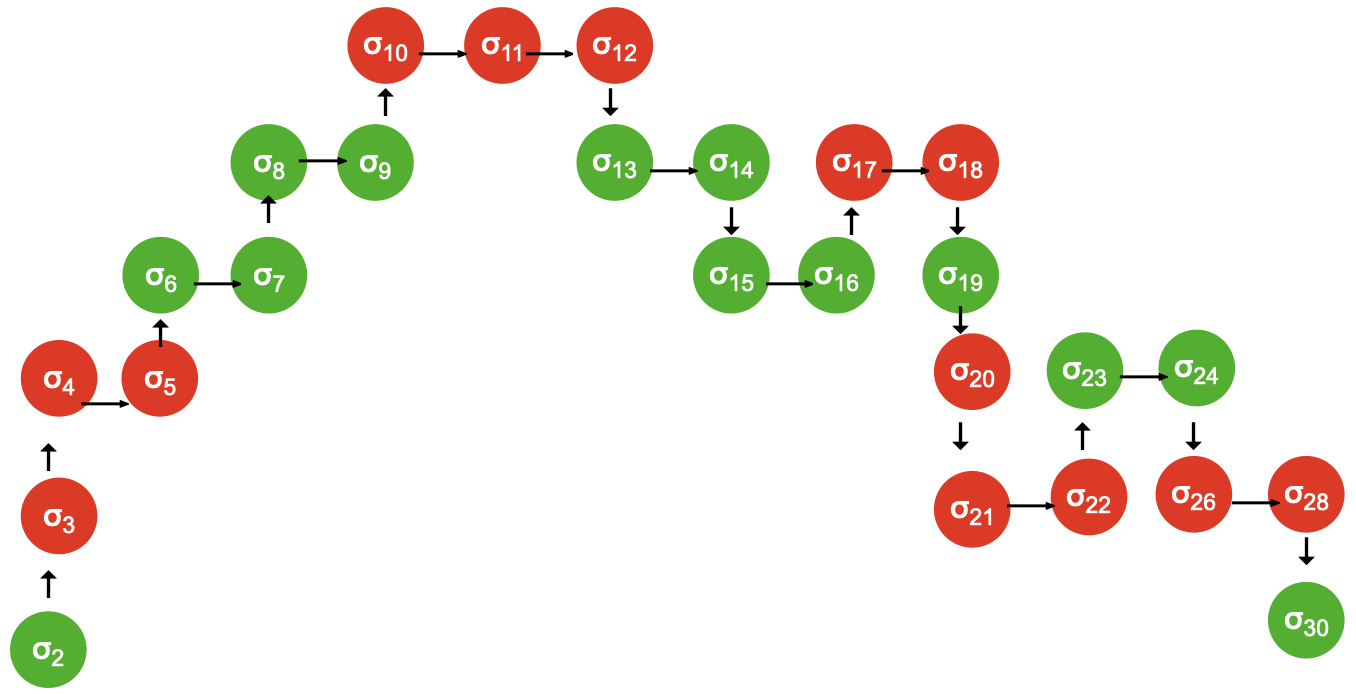
\includegraphics[width=\linewidth]{diagrams/summaryA.png}
} 
\\
\hline \\
the summarised execution:
\\
~ \\
\resizebox{9cm}{!}
{
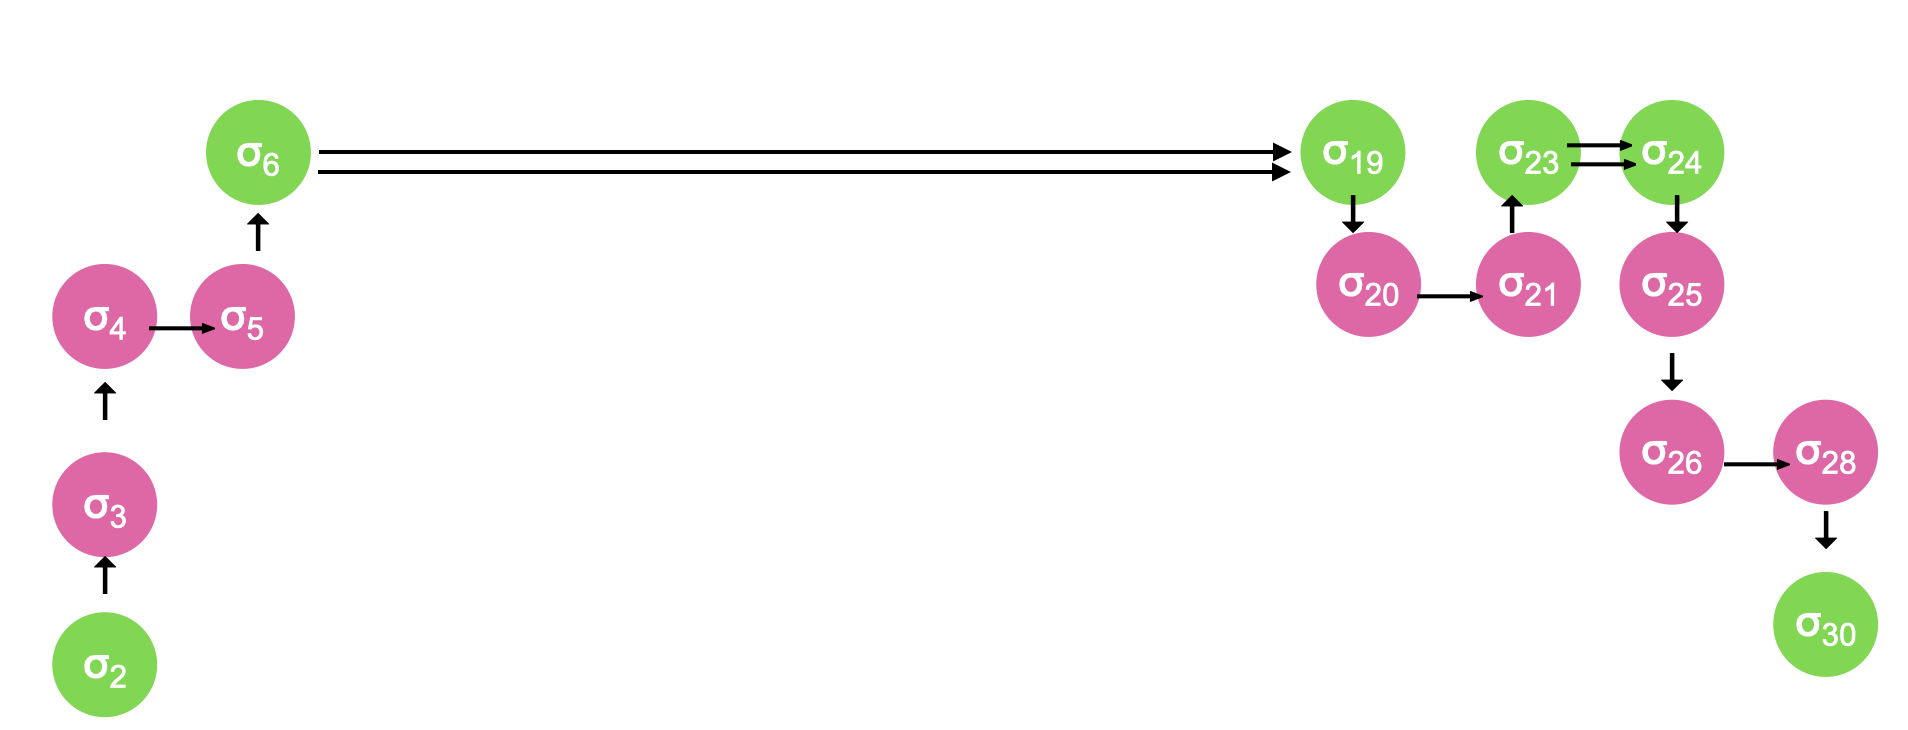
\includegraphics[width=\linewidth]{diagrams/summaryB.png}
} 
\\
\hline \hline
\end{tabular}
   \caption{Summaries. 
   }
   \label{fig:summaries}
 \end{figure}

The lemma  \ref{lemma:external_exec_preserves_more} describes how an encapsulated assertion $A$ is preserved during an execution, provided that all finalizing internal executions preserved it. 
It will be used in the proof of soundness of the rule {\sc{ExtCall\_WithSpec\_Weak}}\footnoteSD{perhaps also {\sc{ExtCall\_WithSpec\_Strong}}}


%\begin{auxLemma}
%\label{lemma:external_exec_preserves}[Preservation of Encapsulated Assertions]
%For any module $M$, modules $\Mtwo$, variables $\overline x$, and addresses $\overline \alpha$,
% states $\sigma\bd$, $\sigma$, and $\sigma'$, and assertions $A$, $A'$:
%
%Assume that $M \models \encaps A \   \wedge  \ A'\txteq A[\overline{\alpha/x}]\  \wedge \ fv(A)=\emptyset \  \wedge \ 
%M, \sigma \models  A' $. Then
%
%\begin{itemize}
%\item
%$   \leadstoBoundedThreeStarExt {\Mtwo\cdot M} {\sigma\bd}  {\sigma}  {\sigma'} 
%\ \ \Longrightarrow \ \ \ M, \sigma' \models A'$
%\item
%$ \leadstoBoundedThreeStarExt {\Mtwo\cdot M} {\sigma\bd}  {\sigma}  {\sigma'} \ \mbox{as a return from a method}
%\ \ \Longrightarrow \ \ \ M, \sigma' \models A'$
%\item
%\end{itemize}
%\end{auxLemma}

 


\begin{auxLemma}
\label{lemma:external_exec_preserves_more}[Preservation of Encapsulated Assertions]
For any module $M$, modules $\Mtwo$, variables $\overline x$, and addresses $\overline \alpha$,
 states $\sigma\bd$, $\sigma$, and $\sigma'$, and assertions $A$, $A'$, 
assume that

\noindent
 $M \models \encaps A \   \wedge  \ A'\txteq A[\overline{\alpha/x}]\  \wedge \ fv(A')=\emptyset \  \wedge \ 
M, \sigma \models  A' $. Then

\begin{enumerate}

\item
$   \leadstoBoundedThreeStarExt {\Mtwo\cdot M} {\sigma\bd}  {\sigma}  {\sigma'} 
\ \ \Longrightarrow \ \ \ M, \sigma' \models A'$

\item
$M, \sigma  \models \extThis \ \wedge \  \leadstoBoundedThree  {\Mtwo\cdot M} {\sigma} {\sigma}  {\sigma_{1}} \ \wedge
 \ M, \sigma_1 \models \pubMeth \ \wedge\  \leadstoBoundedStarFin {\Mtwo\cdot M} {\sigma_1}  {\sigma_2}    \ \ \wedge$\\
$ M, \sigma_2 \models A' \ \wedge \ 
  \   \leadstoBounded  {\Mtwo\cdot M} {\sigma_2}      {\sigma'}$\\
 $\Longrightarrow $
\\
$M, \sigma' \models A' $

\item
$ \WithExtPub {\Mtwo\cdot M} {\sigma\bd}  {\sigma}  {\sigma'} {\sigma_1...\sigma_n}\ \ \wedge $\\
 $\strut \ \ \ \  \  \forall i\in [1..n]. \forall \sigma_{f}.[ \ \  M, \sigma_i \models A'  \ \wedge \  \leadstoBoundedStarFin {M\cdot \Mtwo}  {\sigma_i}  {\sigma_{f}} \ 
\Longrightarrow \  M, \sigma_f \models A' \ ]$\\
$\Longrightarrow $
\\
$M, \sigma' \models A' $
\end{enumerate}

TOTHINK: Do we also need that $A$ is a module invariant?
\end{auxLemma}




\subsection{A well-founded ordering}
\label{sect:prove:wellfounded}

We will prove soundness by well-founded induction.
% \footnote{This kind of induction is described in \texttt{https://en.wikipedia.org/wiki/Well-founded\_relation.}}
We start by designing a well--founded ordering. 



{
\begin{definition}
For a module $M$, and modules $\Mtwo$,   we define a measure, $\measure {A, \sigma,A',A''} {M,\Mtwo} $, and based on it, a well founded ordering $(A_1,\sigma_1,A_2, A_3) \ll_{M,\Mtwo}  (A_4,\sigma_2,A_5,A_6)$
as follows:
\begin{itemize}
\item
 $\measure {A, \sigma,A',A''} {M,\Mtwo} \  \ \triangleq \ \  (m, n)$,  \ \ \  where
\begin{itemize}
\item
$m$ is the minimal number of execution steps so that $ \leadstoBoundedStarFin {M\cdot \Mtwo} {\sigma}    {\sigma'}$  for some $\sigma'$, {and $\infty$ otherwise}.
 \item
  $n$ is minimal depth of all proofs of $M \vdash \quadruple {A} {\sigma.\prg{cont}} {A'} {A''} $.
\end{itemize}
 \item
 $(m,n) \ll (m',n')$\ \  \ \ $\triangleq$ \ \  \ \ $ m<m'\vee  (m=m'  \wedge n < n')   $.
\item
$(A_1,\sigma_1,A_2, A_3) \ll_{M,\Mtwo}  (A_4,\sigma_2,A_5, A_6)$  \  \  $\triangleq$ \ \ 
$\measure {A_1, \sigma_1,A_2, A_3} {M,\Mtwo}  \ll \measure {A_4, \sigma_2,A_5. A_6} {M,\Mtwo} $
\end{itemize}
\end{definition}
}


\begin{auxLemma}
\label{lemma:normal:two}
For any modules $M$ and $\Mtwo$,  the relation $\_ \ll_{M,\Mtwo}  \_$ is well-founded.
\end{auxLemma}

%%%

  %%%%%%%%%%%%%%%%%%%%%%%%%%%%%%%%%%%%%%%%%%%%%%%%%%%

\subsection{ Soundness of  Hoare Quadruples Logic}
\label{sect:prove:sound:quadruples}
We now prove soundness of the inference system $M \vdash  \quadruple A {stmt} {A'} {A''}$:


\begin{theorem}
\label{t:quadruple:sound}
For module  $M$ % and $\Mtwo$, 
such that  $\vdash M$, and for any assertions $A$ and $A'$, and state  $\sigma$, we have

\begin{center}
$M\ \vdash\  \quadruple {A} {\sigma.\prg{cont}} {A'} {A''}$ \ \ \ \ implies \ \ \ \ $M\ \modelsD\  \quadruple {A} {stmt} {A'} {A''}$
\end{center}

\end{theorem}

\noindent
\vspace{.2cm}
  {\textbf{Proof Sketch}} 


\noindent
Take any $M$, $\Mtwo$, with\\ 
$\strut \ \ \hspace{2.3cm} \ \ (1) \ \ \vdash M $.
\\
We will prove that\\
$\strut \ \ \hspace{2.3cm} \ \ (*)\ \ \forall \sigma, A, A', A''.$\\
$\strut \ \ \hspace{2.3cm} \ \ \ \ \  \ \ [ \ M\ \vdash\  \quadruple {A} {\sigma.\prg{cont}} {A'} {A''}  \ \ \Longrightarrow \ \    M\ \modelsD\  \quadruple {A} {stmt} {A'} {A''}\ ]$.\\
by induction on the well-founded ordering  $\_ \ll_{M,\Mtwo}  \_$.
\\
Take $\sigma$, $A$, $A'$, $A''$, $\overline z$, $\overline \alpha$, $\sigma'$, $\sigma''$  arbitrary. Assume that\\
$\strut \ \ \hspace{2.3cm} \ \ (2) \ \ M\ \vdash\  \quadruple {A} {\sigma.\prg{cont}} {A'} {A''}$\\
$\strut \ \ \hspace{2.3cm} \ \ (3) \ \ \overline z = \fv(A)\setminus \vs(\sigma.\prg{cont})$\\
$\strut \ \ \hspace{2.3cm} \ \ (4) \ \ \satDAssertFrom M  \sigma k   A[\overline{\alpha/z}]$\\
To show\\
$\strut \ \ \hspace{2.3cm} \ \ (\alpha) \ \    \leadstoBoundedStarFin {\Mtwo\cdot M}  {\sigma}  {\sigma'}\ \ \Longrightarrow\ \     \satDAssertFrom M  {\sigma'} k   A'[\overline{\alpha/z}]$\\
$\strut \ \ \hspace{2.3cm} \ \ (\beta) \ \    \leadstoBoundedStarFin {\Mtwo\cdot M}  {\sigma}  {\sigma''}\ \ \Longrightarrow\ \     \satDAssertFrom M  {\sigma''}  k  \extThis \rightarrow A''[\overline{\alpha/z}]$
 
 \vspace{.2cm}
\noindent
We proceed by case analysis on the  rule applied in the last step of the proof of (2).

\begin{description} 
 
 \item[{\sc{mid}}] 
 
 By Theorem \ref{l:triples:sound}.

\newcommand{\SPS}{\strut \ \ \hspace{0.5cm} \ \ }
 
\item[{\sc{sequ}}] 
Therefore, there exist statements $stmt_1$ and $stmt_2$, and assertions  $A_1$, $A_2$ and $A''$, so that $A_1\txteq A$, and $A_2 \txteq A'$, and $\sigma.\prg{cont}\txteq  stmt_1; stmt_2$, and $\overline z = \fv(A) \setminus (\vs(stmt_1) \cup \vs(stmt_2))$, and
the proof of  $(2)$ %$M\ \vdash\  \{\, A \,  \}\ s_1;s_2\  \{\, A' \, \}$ in $P$ 
has as its immediate predecessors proofs for \\
$\SPS (5)\ \ M\ \vdash\  \quadruple {A_1} {stmt_1} {A_2} {A''}$,\ \ \ \  and\\
$\SPS (6)\ \  M\ \vdash\  \quadruple {A_2} {stmt_2} {A_3} {A''}$.

Define $\sigma_1$ as  $\sigma_1 \triangleq \sigma[\prg{cont} \mapsto stmt_1]$.
Therefore,  $(A_1,\sigma_1,A_2, A'') \ll_{M,\Mtwo} (A_1,\sigma,A_3, A'')$. 

\vspace{.1cm}
Proving $(\alpha)$. Assume that $\leadstoBoundedStarFin {\Mtwo\cdot M}  {\sigma}  {\sigma'}$. Then, by lemma \ref{lemma:subexp} we obtain that there exists a $\sigma_1'$ such that $\leadstoBoundedStarFin {\Mtwo\cdot M}  {\sigma_1}  {\sigma_1'}$,
and $\leadstoBoundedStarFin {\Mtwo\cdot M}  {\sigma_2}  {\sigma'}$, where $\sigma_2 \triangleq \sigma_1'[\prg{cont} \mapsto stmt_2]$. Moreover,  $(A_2,\sigma_2,A_3,A'') \ll_{M,\Mtwo} (A_1,\sigma,A_3, A'')$.

We will use the following abbreviations: \\
$\SPS (7)\ \ \overline {z_3}\triangleq\vs(stmt_1)\setminus\vs(stmt_2) \ \ \ \ \ \overline {z_4}\triangleq\vs(stmt_2)\setminus\vs(stmt_1) $.\\
Then we have\\
$\SPS  (8)\ \ \fv(A)\setminus\vs(stmt_1) = \overline {z}\cup \overline{z_4}  \ \ \ \ \ 
\fv(A)\setminus\vs(stmt_2) = \overline {z}\cup\overline{z_3} $.
\\
 From (4), and Lemma \ref{lemma:addr:expr}, we obtain\\ 
 $\SPS (9) \ \ \satDAssertFrom M  {\sigma_1} k   {A_1[\overline{\alpha/z}][\overline{{\interpret {\sigma_1} {z_4}} /z_4}]}$\\
 We apply the induction hypothesis, and obtain\\
  $\SPS (10) \ \ \satDAssertFrom M  {\sigma_1'} k   {A_2[\overline{\alpha/z}][\overline{{\interpret {\sigma_1} {z_4}} /z_4}]}$\\
By Lemmas \ref{l:var:unaffect} and \ref{l:assrt:unaffect} and (7) we have that ${\overline{{\interpret {\sigma_1} {z_4}} /z_4}]}$=${\overline{{\interpret {\sigma_1'} {z_4}} /z_4}]}$=${\overline{{\interpret {\sigma_2} {z_4}} /z_4}]}$, and this, applied to (10) and again with Lemma \ref{lemma:addr:expr} gives us\\
 $\SPS (11) \ \ \satDAssertFrom M  {\sigma_2} k   {A_2[\overline{\alpha/z}]}$\\
We apply Lemma \ref{lemma:addr:expr} again, and obtain\\
 $\SPS (12) \ \ \satDAssertFrom M  {\sigma_2} k   {A_2[\overline{\alpha/z}][{\overline{{\interpret {\sigma_2} {z_3}} /z_3}}]}$\\
 We apply again the induction hypothesis, and obtain\\
  $\SPS (13) \ \ \satDAssertFrom M  {\sigma'} k   {A_3[\overline{\alpha/z}][\overline{{\interpret {\sigma_1} {z_3}} /z_3}]}$\\
By similar argument as earlier, we obtain:\\
 $\SPS (\alpha') \ \ \satDAssertFrom M  {\sigma'} k   {A_3[\overline{\alpha/z}]}$ 
 
 \vspace{.1cm}
Proving $(\beta)$.
Let us now take an arbitrary $\sigma''$ such that   $\leadstoBoundedStar  {\Mtwo\cdot M}  {\sigma}  {\sigma''}$. By
lemma  \ref{lemma:subexp}, either $\leadstoBoundedStar  {\Mtwo\cdot M}  {\sigma_1}  {\sigma''}$ or
$\leadstoBoundedStar  {\Mtwo\cdot M}  {\sigma_2}  {\sigma''}$. 

In the first case, where $\leadstoBoundedStar  {\Mtwo\cdot M}  {\sigma_1}  {\sigma''}$ we apply the inductive hypothesis, and obtain $(\beta')$, ie that \ \ $ M, \sigma'' \models \extThis \rightarrow A''[\overline{\alpha/z}]$.

 The second case is analogous.
 
  \item[{\sc{combine}}] ... easy ...
  
 \item[{\sc{consequ}}] ... using Lemma \ref{l:shallow:deep} part \ref{fourSD}  and axiom \ref{lemma:axiom:enc:assert:ul}

%
%
\item[{\sc{Call\_Int}}]
 
 Therefore, there exist $u$, $y_o$, $C$, $\overline y$,  $A_1$ and $A_2$ such that \\
 $\SPS (5) \ \ \sigma.\prg{cont}\txteq u=y_0.m(\overline y)$,  \ \ \ \ $\overline z = \fv(A)\setminus \{ u, y_0, ... y_n \}$
\\ 
$\SPS (6) \  \ \promises  M {\mprepostN {A_{pre}}{D}{m}{y}{D}{A_{post}} {A_{mid}}}$, \\
$\SPS (7) \  \ A \txteq y_0:D ,\overline {y:D}\ \wedge \  A_{pre}[y_0/\prg{this}],\ \  \ \ 
A'  \txteq A_{post}[y_0/\prg{this},u/res],\ \  \  A'' \txteq  A_{mid}$. 
\\
Also, \\
$\SPS (8) \ \ \leadstoBounded  {\Mtwo\cdot M}  {\sigma}  {\sigma_1}$, \\
 where $\sigma_1\triangleq (\PushSLong { (\prg{this}\mapsto {\interpret{\sigma} {y_0}},{\overline{y \mapsto {\interpret{\sigma} {y}}}})}\sigma [\prg{cont}\mapsto stmt_m]$, and where 
  $\prg{mBody}(m,D,M)=\overline{y:D}\{\    stmt\_m\ \}$ .\\
By (1), (7), and definition of $\vdash M$ in Section \ref{sect:wf}, we obtain\\
$\SPS (9) \ \ M \vdash  \quadruple { \ \prg{this}:D,\overline{y:D}\, \wedge\, A_{pre}\  } {\ stmt\_m } {\ A_{post}\ } {A_{mid}}$.\\
From (8) and (9) we obtain  \\
$\SPS (10) \ \ (\prg{this}:D,\overline{y:D}\, \wedge\, A_{pre},\sigma_1,A_{post}, A_{mid}) \ll_{M,\Mtwo} (A,\sigma,A', A'')$. 
\\
By (1), (7) and Lemma   \ref{l:shallow:deep} part \ref{fiveSD}, we obtain\\
$\SPS (11) \ \  \satDAssertFrom M  {\sigma_1} {(k+1)}   {\prg{this}:D,\overline{y:D}\, \wedge\, (A_{pre}[\overline{\alpha/z}])}$.

 \vspace{.1cm}
Proving $(\alpha)$. Assume that   $\leadstoBoundedStarFin  {\Mtwo\cdot M}  {\sigma}  {\sigma'}$. Then, by the operational semantics, we obtain that 
there exists state $\sigma_1'$, such that \\
$\SPS (12) \ \ \leadstoBoundedStarFin  {\Mtwo\cdot M}  {\sigma_1}  {\sigma_1'}$ \\
$\SPS (13) \ \ \sigma'=(\sigma_1'\popSymbol)[u \mapsto {\interpret {\sigma_1'} {res}}][\prg{cont}\mapsto skip]$.\footnote{TODO: define $skip$ as a possible statement, and define $\popSymbol$ as an operation that pops a frame -- both straightforward.}
\\
Using (9), (10), and because by Barendregt we can assume that $\fv(A)\cap \vs(stmt\_m) = \emptyset$, we can apply the inductive hypothesis, and obtain\\
$\SPS (14) \ \  \satDAssertFrom M  {\sigma_1'} {(k+1)}   {\prg{this}:D,\overline{y:D}\, \wedge\, (A_{post}[\overline{\alpha/z}])}$.
\\
By (13), (14) and Lemma  \ref{l:shallow:deep} part \ref{fiveSD}\footnote{TODO: check whether it needs some more, eg that in the penultimate frame in $\sigma_1'$ variable $y_0$ points to \prg{this} of the top in $\sigma$}, we obtain\\
$\SPS (\alpha') \ \  \satDAssertFrom M  {\sigma'} {k}   {A_{post}[y_0/ \prg{this},u/res][\overline{\alpha/z}]}$.\\
and using (7) we are done.

 \vspace{.1cm}
Proving $(\beta)$. Similar.

\item[{\sc{Call\_Int\_Adapt}}]
% 
% From (3), (11) and lemma \ref{lemma:push}.\ref{pushOne}  we obtain that \ \ \  $ (15) \ \ M, \sigma_1 \models \overline{y:C}\, \wedge\, A_1$.\footnote{{Here some renaming needed,  but easy to do0.}}
% 
% From (10), (11) and (12) we obtain that $( \prg{this}:\prg{C}\, \wedge\, \overline{y:C}\, \wedge\, A_1,\sigma_1,A_2) \ll_{M,\Mtwo,P} (A,\sigma,A')$. By induction hypothesis, (15) and (13) we obtain that (16) $M,\sigma_2 \models A_2$.
% 
% By (14) and lemma  \ref{lemma:push}.\ref{pushTwo}  we obtain that 
%\ \ $M,\sigma' \models \PushAS  {y} {A_2[ u/res]}$. \. With (9) this gives $M,\sigma' \models A'$.
%
%\item[ {\sc{Call\_B}}]
%
%Therefore, there exist $u$, $y_o$, $C$, $\overline y$,  $A_1$ and $A_2$ such that \\
%%\begin{tabbing}
%6)\ $\sigma.\prg{cont}\txteq u=y_0.m(\overline y)$,   \hspace{2cm}
% (7)\ $A \txteq y_0:C  \ \wedge\ \overline {y:C}\ \wedge \  (\PushAS  {y} {A_1})$, 
%\\
% (8)\ $\promises M {\mprepost{A_1}{C}{m}{y}{C}{  {A_2}} }$,    \hspace{1cm}
% (9)\ $A' \txteq  {\PushAS  {y} {(A_2[ u/res])}}$. 
%% \end{tabbing}
%
%By (1), (8), and definition of $\vdash M$ in Section \ref{sect:wf}, we obtain that   $\prg{mBody}(m,C,M)=\overline{y:C}\{\  s \ \}$ and that\\
%(10)   ${\hproves{M} { \ \prg{this}:\prg{C}\, \wedge\, \overline{y:C}\, \wedge\, A_1\  } {\ s\ } {\ A_2\ } }$ is proven in $P$.
% 
% By the operational semantics, we obtain that there exist states $\sigma_1$, and $\sigma_2$, such that \\
% (11)\ $\sigma_1=\sigma.PUSHFRAME(\prg{this}, {\overline y} \mapsto \overline{\interpret {\sigma} y},\prg{cont} \mapsto s) $, TODO   \hspace{1cm}
%   (12)\ $\leadstoBounded  {\Mtwo\cdot M}  {\sigma}  {\sigma_1}$ \\
% (13)\ $\leadstoBoundedStarFin {\Mtwo\cdot M}  {\sigma_1}  {\sigma_2}$,   \hspace{3cm}
% (14)\ $\sigma'=\sigma_2[...]$ TODO.
% 
% From (3), (11) and lemma \ref{lemma:push}.\ref{pushOne}  we obtain that \ \ \  $ (15) \ \ M, \sigma_1 \models \overline{y:C}\, \wedge\, A_1$.\footnote{{Here some renaming needed,  but easy to do0.}}
% 
% From (10), (11) and (12) we obtain that $( \prg{this}:\prg{C}\, \wedge\, \overline{y:C}\, \wedge\, A_1,\sigma_1,A_2) \ll_{M,\Mtwo,P} (A,\sigma,A')$. By induction hypothesis, (15) and (13) we obtain that (16) $M,\sigma_2 \models A_2$.
% 
% By (14) and lemma  \ref{lemma:push}.\ref{pushTwo}  we obtain that 
%\ \ $M,\sigma' \models \PushAS  {y} {A_2[ u/res]}$. \. With (9) this gives $M,\sigma' \models A'$.
%
%\item[${\sc{ExtCall\_WithSpec\_Weak}}$]
%
%Therefore, there exist $u$, $y_o$, $C$, $\overline y$,  $A_1$ and $A_2$ such that \\
%(6)\ $\sigma.\prg{cont}\txteq u=y_o.m(\overline y)$,  \hspace{2cm}
% (7)\ $A \txteq   { \external{y_0} }\, \wedge \, \overline {x:C}  \, \wedge \,  {\PushAS  {y}{  A_1} \,   \wedge \,  \PushAS {y}{\extract{M}}}\ $,\footnote{{There is a relation between $A_1$ and  $\extract{M}$ -- we should revisit that. 
% But the proof structure is unaffected.}}
%\\
% (8)\ $\promises M   {\TwoStatesN {\overline {x:C}} {A_2}}$ \ \ proven in $P$,   \hspace{1cm}
% (9)\ $A' \txteq \PushAS  {y} { A_2}$. 
% \\
% %By (8) and (1), and axiom \ref{lemma:axiom:enc:assert}, we obtain \ \ \ (10) \ $M \models \encaps{A}$.
%% \\
% By the operational semantics, we obtain that there exist states $\sigma_{e\_1}$, and $\sigma_{e\_1}$, such that \\
% (11)\ $\sigma_{e\_1}=\sigma ...[\prg{cont}\mapsto s]... $, TODO   \hspace{1cm}
%   (12)\ $\leadstoBounded  {\Mtwo\cdot M}  {\sigma}  {\sigma_{e\_1}}$ \\
% (13)\ $\leadstoBoundedStarFin {\Mtwo\cdot M}  {\sigma_{e\_1}}  {\sigma_{e\_2}}$,   \hspace{1cm}
% (14)\ $\sigma'=\sigma_{e\_1}[...]$ TODO.
%\\
%By (8) and (2) we obtain that there exists an $A_0$ \\
%(15)\ $\TwoStatesN {\overline {x:C}} {A_0}  \in HS(M)$\\ and \\
% (16) $M \vdash A_1 \rightarrow A_0$ proven in $P$ \ \ \ \ \ \ \  (17) $M \vdash A_0 \rightarrow A_2$ proven in $P$ \\
%By (7) and (3) we obtain \ \ 
%(18) $M, \sigma \models \extThis$, %\hspace{2cm) 
%\\
%By (3), (7), (11), (16) and lemma  \ref{lemma:push}.\ref{pushOne} , we get \ \ \ \  (19) $M, \sigma_{e\_1} \models  {  A_0} \,   \wedge \,  {\extract{M}} \, \wedge \, 
%\overline{ {\interpret \sigma x} : C}$.
%\\
%By (8) and (1), and axiom \ref{lemma:axiom:enc:assert}, we obtain \ \ \ (20) \ $M \models \encaps{{  A_0} \,   \wedge \,  {\extract{M}} \, \wedge \, 
%\overline{ {\interpret \sigma x} : C}}$.
%\\
%By (4) and (18), we can apply auxiliary lemma 
%\ref{lemma:external_breakdown} and break down the execution from $\sigma_{e\_1}$ to  $\sigma_{e\_2}$ into the internal and external executions as follows:
%%For any module $M$, modules $\Mtwo$, states $\sigma$ and $\sigma'$:
%\\
%There exists $ p,q\in \mathbb{N},  \sigma_1, ... \sigma_q \in States, m_1,...m_p, n_1, ... n_p \in \mathbb{N}.$, such that \\ 
%% $\strut \ \ \ \ \ \ \ \ \ \ [  $ \\
%$\ \strut \ \ (21) \ \sigma_1=\sigma_{e\_1} \ \ \wedge\ \  \sigma_p=\sigma_{e\_2}\ \  \wedge\ \ \forall i\in [1..q).[\   \leadstoOrig {M\cdot \Mtwo}  {\sigma_i}  {\sigma_{i+1}}\  ] \  \ \ \wedge$\\
%$\ \strut \ \ (22) \ \ m_1=1 \ \wedge\ n_p=q+1 \  \wedge\ \forall i\in[1..p).[  \  m_i < n_i < m_{i+1}  ] \ \wedge \ m_p<n_p\ \ \wedge  $\\
%$\ \strut \ \ (23) \ \ \forall i\in[1..p].\forall j\in [m_i..n_i)[\   M,\sigma_j \models \external {\texttt{this}} \ ] \  \ \ \wedge$\\
%$\ \strut \ \ (24) \ \ \forall i\in[1..p). [ \ M,\sigma_{n_i} \models \internal {\texttt{this}}   \ \wedge \ \ 
% \leadstoBoundedStarFin {M\cdot \Mtwo}  {\sigma_{n_{i}}}  {\sigma_{m_{i+1}-1}} \ ] $ \\
%%$\strut \ \ \ \ \ \ \ \ \ \ ]$
%From (12), and (21) we obtain that\\
%$\ \strut \ \ (25)\   \forall i\in[1..p). [ \ \leadstoBoundedStar {M\cdot \Mtwo}  {\sigma} {\sigma_{n_{i}}} \ ]$\footnote{needs so tidying up, but easy}
%\\
%From  (24) and (15) and (1) we obtain that\\
%$\ \strut \ \ (26)\ \forall i\in[1..p). [ \ M\vdash \{ \, A_0  \}\, {\sigma_{n_{i}}.\prg{cont}}  \{ \, A_0 \}\ \  \mbox{ is proven in } P \ ]$\footnote{{because of the design issue it could be that we would have $\extract M$ rather than $A_0$ -- but this is an orthogonal dewsign question, and the soundness argument would hold either way.}}, \\
%\\
%From (25) and (26) we obtain that\\
%$\ \strut \ \ (27)\   \forall i\in[1..p).[ \ ( A_0, \sigma_{n_{i}}, A_0 ) \ll_{M,\Mtwo,P}  A, \sigma, A' )\ ]$
%\\
%From (24), (26), (27), and the induction hypothesis, we obtain\\
%$\ \strut \ \ (28)\    \forall i\in[1..p).[ \ \  M, \sigma_{n_{i}} \models A_0 \ \Longrightarrow \ \ M, \sigma_{m_{i+1}-1} \models A_0 \ \ ]$.\\
%We apply auxiliary lemma \ref{lemma:external_exec_preserves} on (19), (20) (21), (22), (23), (28), and obtain\\
%$\ \strut \ \ (29) \   M, \sigma_{e\_2} \models A_0$.\\
%We now apply lemma \ref{lemma:push}.\ref{pushTwo} on (29) and  (14) and obtain\\
%$\ \strut \ \ (30) \   M, \sigma'  \models \PushAS  {y}{A_0}$.
%We apply (17) on (30) and obtain\\
%$\ \strut \ \ (30) \   M, \sigma'  \models \PushAS  {y}{A_2}$.
\end{description}
\noindent
\vspace{.1cm}
  {\textbf{End Proof Sketch}} 

\vspace{1cm}

  %%%%%%%%%%%%%%%%%%%%%%%%%%%%%%%%%%%%%%%%%%%%%%%%%%%
  \subsection{Soundness of the overall system}
\label{sect:prove:triples:overall}
Finally, we can now prove soundness of the overall system

\begin{theorem}[Soundness]
\label{thm:soundness}
Assume an \SpecO proof system, $\proves{M}{A}$, 
an encapsulation inference system, $\proves{M}{\encaps{A}}$,
% Axiom xx, and 
 and  that on top of these systems we built
 the \SpecLang logic according to zzzz,  then, for    all modules $M$, and all \SpecLang specifications  $S$:
 
 $$\proves{M}{S}\ \ \ \ \ \ \ \mbox{implies}\ \ \ \ \ \  \ \ \ \satisfies{M}{S}$$
\end{theorem}

\begin{proof}
% follows from earlier theorem and the axiom.
TODO: We will make a similar argument as for method calls in previous subsection, and will be using AuxLemma 8.4
% by induction on the derivation of $\proves{M}{S}$.
\end{proof}
 


Theorem. \ref{thm:soundness} demonstrates 
 that the   \SpecLang logic is sound with respect to the semantics of \SpecLang specifications.
 The \SpecLang logic parametric wrt to the algorithms for proving validity of assertions
 $\proves{M}{A}$, and 
 assertion encapsulation ($\proves{M}{\encaps{A}}$), and is sound
 provided that these two proof systems are sound.
